\subsection{Le langage SFC}
Le langage SFC (\textit{Sequential Function Chart}) est un langage graphique permettant de décrire le comportement d'un système automatisé. Il est basé sur le formalisme des GRAFCET (\textit{GRAphe Fonctionnel de Commande Etape Transition}).

\UPSTIremarque{Bien qu'ils soient très similaires à première vue, le GRAFCET est un langage  destiné à la spécification alors que le SFC est un langage destiné à la programmation.}

\begin{UPSTIinfor}{Rappels sur le SFC}
Un graph SFC consiste en une succession d'\textbf{étapes} et de \textbf{transitions}. A l'origine, une seule étape initiale est active. A chaque cycle, les transitions sont évaluées. Une transition est dite \textbf{franchissable} si sa \textbf{réceptivité} est ~TRUE~ et que l'étape qui la précède est active.
Si une transition est franchissable, elle est franchie et l'étape suivante devient active.
Lorsqu'une étape est active, elle exécute l'ensemble des \textbf{actions} qui lui sont associées.

Rappel de vocabulaire : 
\begin{description}
    \item[Étape] : Une étape est un ensemble d'actions qui s'exécutent en parallèle. Une étape est représentée par un rectangle. 
    \item[Transition] : Une transition est un ensemble de conditions qui doivent être vérifiées pour passer d'une étape à une autre. Une transition est représentée par un trait horizontal. 
    \item[Action] : Une action est une opération élémentaire qui peut être réalisée par le système. Une action est représentée par un rectangle vertical.
    \item[Réceptivité] : Une réceptivité est une condition booléenne qui doit être vérifiée pour qu'une transition soit franchissable.
\end{description}
\end{UPSTIinfor}

\subsubsection{Les actions en SFC}

\begin{wrapfigure}{r}{0.3\linewidth}
    \centering
    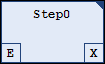
\includegraphics[width=.5\linewidth]{_cds_sfc_step_active.png}
    \caption{Action en SFC}
    \label{fig:ActionSFC}
\end{wrapfigure}
Sous CodeSys, l'activation d'une étape entraîne l'exécution de l'ensemble des actions qui lui sont associées. Elles peuvent être exécutées : 

\begin{enumerate}
    \item Une seule fois à l'activation de l'étape (Les \textbf{Actions d'entrées} -- \textbf{Entry actions}).
    \begin{itemize}
        \item La présence d'une action d'entrée est indiquée par un E dans le coin inférieur gauche de l'étape.
    \end{itemize}
    \item Exécutée à chaque cycle tant que l'étape est active (Les \textbf{Actions actives} -- \textbf{actions}).
    \begin{itemize}
        \item La présence d'une action active est indiquée par un triangle dans le coin supérieur droit de l'étape.
    \end{itemize}
    \item Une seule fois à la désactivation de l'étape (Les \textbf{Actions de sortie} -- \textbf{Exit actions}).
    \begin{itemize}
        \item La présence d'une action de sortie est indiquée par un X dans le coin inférieur droit de l'étape.
    \end{itemize}
\end{enumerate}

A chaque action est associée un qualificatif dont la signification est donnée dans le tableau suivant : 

\begin{center}
    

\begin{tabular}[t]{l|l|p{0.5\linewidth}}
   \textbf{Qualificatif} & \textbf{Nom} & \textbf{Description} \\
    \hline
    N & Non-stored & L'action est exécutée tant que l'étape est active\\\hline
    S0 & Stored & L'action est exécutée dès que l'étape est active. Elle restera active jusqu'à ce qu'elle soit désactivée (même après que l'étape n'est plus active)\\\hline
    R0 & Reset & L'action est désactivée et cesse donc d'être exécutée\\\hline
    L & time Limited & L'action commence son exécution à l'activation de l'étape et s'arrête après un temps défini ou lorsque l'étape est désactivée\\\hline
    D & time Delayed & L'action commence son exécution après un temps défini suivi l'activation de l'étape et s'arrête lorsque l'étape est désactivée\\\hline
   P & Pulse & L'action est exécutée une seule fois à l'activation de l'étape\\\hline
   SD & Stored and time Delayed & L'action commence son exécution après un temps défini suivi l'activation de l'étape, même si cette dernière n'est plus active. L'action s'exécute tant qu'elle n'est pas désactivée (même après que l'étape n'est plus active)\\ \hline
   DS & Delayed and Stored & L'action commence son exécution après un temps défini suivi l'activation de l'étape, si celle-ci est toujours active. L'action s'exécute tant qu'elle n'est pas désactivée (même après que l'étape n'est plus active)\\ \hline
   SL & Stored and time Limited & L'action commence son exécution à l'activation de l'étape et s'arrête après un temps défini ou lorsque l'étape est désactivée. \\
   \hline
\end{tabular}
\end{center}

\subsubsection{Les transitions en SFC}
La réceptivité associée à une transition sous CodeSys peut être vue comme l'appel d'une fonction. En effet, il est possible d'exécuter un algorithme pour évaluer la réceptivité d'une transition.


\subsubsection{Les drapeaux d'un graph SFC}
Les drapeaux sont des variables qui (souvent booléennes) qui permettent le contrôle et le suivi de l'évolution d'un graph SFC. 
Le tableau suivant décrit les principaux drapeaux que nous rencontrerons : 
\begin{center}
    \begin{tabular}[t]{l|p{0.6\linewidth}}
        \hline
        ~SFCInit : BOOL~ & Son passage à ~TRUE~ entraine l'initialisation normalisée du graph SFC et de tous les drapeaux. Tant qu'elle est à ~TRUE~, le graph SFC reste dans son état initial, sans qu'aucune action ne soit exécutée.\\\hline
        ~SFCReset : BOOL~ & Son passage à ~TRUE~ entraine la réinitialisation du graph SFC et de tous les drapeaux. Tant qu'elle est à ~TRUE~, le graph SFC reste dans son état initial et \textbf{l'action associée à l'étape initiale est exécutée}.\\\hline
        ~SFCPause : BOOL~ & Son passage à ~TRUE~ entraine la mise en pause du graph SFC. \\\hline    
        ~SFCTrans : BOOL~ & Passe à ~TRUE~ à chaque franchissement d'une transition. \\\hline
        ~SFCCurrentStep : STRING~ & Contient le nom de l'étape active. Si plusieurs étapes sont active, celui de l'étape la plus à droite. \\\hline
    \end{tabular}
\end{center}

%%% TODO : Notion de grafcet partiel coopérant %%%

